\documentclass[a4paper,12pt,russian]{article}

\usepackage{geometry}
\geometry{a4paper,top=2cm,bottom=2cm,left=2cm,right=2cm} %% отступы и т.п.

%% чтоб работал русский язык
\usepackage[utf8]{inputenc}
\usepackage[russian]{babel}

%% для математических символов
\usepackage{amsmath, amsthm, amssymb}

%% листинги кода
\usepackage{listings}
\usepackage{courier}
\lstset{
  language=c++,
  basicstyle=\footnotesize\sffamily,
  keywordstyle=\bfseries,
  stringstyle=\ttfamily,
  numberstyle=\tiny,
  numbers=left
}

%% картинки
\usepackage[pdftex]{graphicx}
\usepackage[small, bf, labelsep=period]{caption}
\graphicspath{{img/}}
\usepackage{multicol}

%% листинги программ
\usepackage{moreverb}
\usepackage[noend]{algorithmic}
\algsetup{indent=2em, linenosize=\small, linenodelimiter=}

%% чтоб первый абзац был с отступом
\usepackage{indentfirst}

%% всякое для удобства разметки
%\newcommand{\remark}[1]{~~\textit{\textbf{(#1)}}}
\newcommand{\remark}[1]{\footnote{#1}}

\newcommand{\picref}[1]{\textbf{рис.~\ref{#1}}}

\newtheorem*{definition}{Определение}

\begin{document}
\begin{titlepage}
	\begin{center}
		\Large
		Московский~государственный~университет\\
		имени М.В.~Ломоносова\\[0.5em]
		\large
		Факультет~вычислительной~математики~и~кибернетики\\
		Кафедра~системного~программирования
	\end{center}

\vskip 14em
	\begin{center}
		\LARGE
		Дипломная работа\\
		\textbf{``Восстановление определений классов на языке Си++ посредством динамического анализа бинарного кода''}\\
	\end{center}
\vskip 6em
	\begin{flushright}
		\large
		Выполнил~студент 527~группы\\
		Прохоренков~П.В.\\
		\vspace{2cm}
		Научный руководитель\\
		к.ф-м.н, доц. Чернов~А.В.\\
\end{flushright}
\vfill
	\begin{center}
		\Large
		Москва\\
		2009
	\end{center}
\end{titlepage}

\tableofcontents

\newpage

\addcontentsline{toc}{section}{Введение}
\section*{Введение}
\emph{Обратная инженерия} является процессом анализа системы, имеющим 2 цели: восстановление компонент системы и их взаимных связей, и создание описания системы в другой форме с более высоким уровнем абстракции

\emph{Декомпиляция} представляет собой составную часть процесса обратной инженерии, это трансформация программы, которая восстанавливает код на языке высокого уровня по исполняемому файлу программы, ассемблерному коду, либо по любому представлению низкого уровня.
Декомпиляция является обратным преобразованием к компиляции.

Декомпиляция может использоваться для
\begin{itemize}
\item{\textbf{Поиска ошибок, уязвимостей, вредоносного кода}} Например, в более не поддерживаемом программном обеспечении, поставляемом в без исходных кодов.
\item{\textbf{Верификации}} С помощью декомпиляции задачу верификации двоичного кода можно свести к задаче верификации кода на языке высокого уровня.
\item{\textbf{Восстановления алгоритмов работы}}
\item{\textbf{Обеспечения совместимости программ}} Например, создание модулей расширения для программ, к которым не существует доступных описаний двоичных интерфейсов.
\item{\textbf{Оптимизации}} Например, старая программа, скомпилированная для старого процессора, может быть перекомпилирована под новый с использованием всех существующих оптимизаций.
\item{\textbf{Переноса на другую платформу}} После декомпиляции кода, можно скомпилировать его для другой платформы, для которой существует компилятор выходного языка декомпилятора.
\item{\textbf{Восстановления утраченного исходного кода}}
\item{\textbf{Восстановления протоколов обмена программ, исходные коды которых утрачены}}
\end{itemize}

В данной работе будет рассматриваться декомпиляция программ, изначально написанных на языке Си++.
Язык Си++ является универсальным языком с поддержкой объектно-ориентированной парадигмы программирования \cite{strstr}. Этот язык получил широкое распространение, и существует множество программ, написанных на нем.

Одной из подзадач декомпиляции является восстановление типов данных высокого уровня, как базовых, так и производных.
В программах на языках высокого уровня разработчику ПО доступно множество различных типов данных.
В их число входят и составные типы данных, во многих случаях размещаемые в динамической памяти.

В ассемблере отсутствует информация о структурах данных, использованных исходной программой.
Все операции доступа к полям данных структур представляются в виде операций с отдельными ячейками памяти с использованием адресной арифметики.
К примеру, в приведённом коде
\begin{lstlisting}
struct {
  int a;
  int b;
} s;

void f() {
  s.b = 1;
}
\end{lstlisting}
Операция доступа к полю \texttt{b} структуры \texttt{S} на платформе x86 может иметь следующий вид:
\begin{lstlisting}[language={[x86masm]Assembler}]
movl $s, %eax
movl 1, 4(%eax)
\end{lstlisting}
Таким образом, утрачивается информация о структурах данных.
Использование статических методов анализа для решения задачи восстановления составных типов осложняется тем, что необходимо проведение анализа потоков данных и управления, точное восстановление которых статическими методами невозможно.

Динамический анализ во многих случаях позволяет получать недостающую информацию. Но к числу его недостатков надо отнести необходимость запуска исследуемой программы.
Это требует получения входных данных, в обработке которых будут задействованы все интересующих исследователя участки кода.
Также, в некоторых случаях необходимы большие вычислительные ресурсы из-за накладных расходов инструментария анализа.

Знание иерархии классов, используемых в анализируемой программе может иметь большое значение для специалиста. Например, многие алгоритмы могут быть распознаны по используемым в них структурам данных.

Данная работа посвящена восстановлению иерархий классов по бинарному коду в программах, написанных на языке Си++.
Восстановление проходит при помощи динамического анализа программы.

\newpage
\section{Постановка задачи}
Требуется разработать и реализовать инструментальное средство, использующее методы динамического анализа для восстановления иерархии классов, используемых в анализируемой программе.
Результатом работы средства должно являться наиболее полно восстановленное:
\begin{enumerate}
\item Множество классов.
\item Частичное отношение наследования между классами.
\item Таблица виртуальных функций для каждого из классов.
\item Список полей для каждого из классов.
\item Частичное отношение ассоциации между классами.
\end{enumerate}

При реализации необходимо использовать инструментальную среду для динамического анализа программ Valgrind.
Требуется реализовать поддержку языка Си++ для написания инструментов в среде Valgrind.

\newpage
\section{Методы и средства обратной инженерии классов по бинарному коду}
Задаче восстановления иерархий классов уделено недостаточно внимания в литературе.
Существует несколько публикаций, затрагивающих вопрос восстановления иерархий с использованием статического анализа исполняемых файлов.

Работа ``Reversing C++'' \cite{reversing_cpp} описывает методы такого восстановления применительно к коду, сгенерированному компилятором Microsoft Visual C++.
Авторы использовали среду IDA Pro \cite{ida_pro} для получения ассемблерного кода, и реализовали свой инструмент в виде подключаемого модуля для этой среды.
Метод восстановления использовал многие особенности компилятора, такие как передача указателя \texttt{this} через регистр \texttt{ecx}, принятую в компиляторе схему декорирования имён функций, расположение в памяти объектов полиморфных классов.
Описанный метод позволяет восстанавливать полную иерархию классов, если в исполняемом файле присутствует \emph{информация о типах времени выполнения} (\emph{Run-time type info, RTTI}).
Такая информация содержит все данные о наследовании классов и их именах, поэтому правильный разбор структур данных позволяет восстанавливать иерархии классов с большой точностью.
Более сложный случай, который рассмотрен в статье, это случай, когда такая информация отсутствует в исполняемом файле.
В таком случае, восстановление использует данные о таблицах виртуальных функций и конструкторах классов.
В конструкторе унаследованного класса должны быть вызваны конструкторы родительских классов.
Эта информация позволяет восстанавливать некоторую часть иерархии.


Работа ``Using a decompiler for real-world source recovery`` \cite{real_decomp} описывает применение существующих инструментов для декомпиляции программ.
Авторы работы описывают опыт, полученный при декомпиляции реального приложения.
В качестве инструментальный средств были использованы дизассемблер IDA Pro \cite{ida_pro} и декомпилятор Boomerang \cite{boomerang}.
Также, многие участки декомпилированного кода требовали редактирования вручную для улучшения читабельности, либо для приведения кода в компилируемый вид.
Полная иерархия классов была восстановлена на основе информация о типах времени выполнения.
При этом никаких инструментальных средств не было использовано, и разбор всех структур данных и построение иерархии авторы выполнили вручную.

Также, есть работы, посвящённые применению динамического анализа для установления различных свойств программ.

Работа \cite{typechecking} описывает инструмент для динамической проверки программ на языке \texttt{Си}, называемый \texttt{Hobbes}.
Многие важные программные системы написаны на языке \texttt{Си}.
Язык \texttt{Си} не предоставляет строгих гарантий безопасности типов, и многие типичные ошибки разработчиков ПО не отлавливаются компилятором. Такие ошибки проявляют себя только во время исполнения в виде непредсказуемого поведения программы.
Описываемый инструмент интерпретирует откомпилированную программу, отслеживает информацию о типах во всех участках памяти и регистрах и позволяет находить множество ошибок, связанных с типами данных.

Ошибка доступа к памяти происходит, когда программа производит доступ к неверному участку памяти.
Два примера таких ошибок это чтение из памяти, которая не была выделена и чтение из выделенной, но не проинициализированной памяти.

Ошибка типа возникает, когда операция производится с операндами, чьи типы не совместимы с операцией.
Сложение указателя со значением с плавающей запятой, вызов функции с неверным числом аргументов, разыменование значения типа \texttt{int}, как указателя --- все это ошибки типов.

Нахождение ошибок такого рода, используя статические методы анализа сильно затруднено тем, что необходимо точно находить множества значений переменных.
На данный момент не существует точных методов решения этой задачи.

Для того, чтобы отследить эти ошибки, инструмент поддерживает теневые значения, содержащие признак выделенности и тип для всех значений, доступных целевой программе, которые обновляются и проверяются во время работы программы.
Например, результат команды \texttt{mul} --- всегда целое значение, результат \texttt{lea} --- указатель, тип результат инструкции \texttt{add} определяется типами её аргументов.
Поддерживается возможность получения изначальной информации о типах с использованием исходного кода анализируемой программы.

Инструментальное средство \texttt{Hobbes} состоит из двух отдельных частей: интерпретатора кода \texttt{x86}, который обеспечивает работу целевой программы и инструмент для проверки типов --- модуль, вызываемый интерпретатором, когда происходят зарегистрированные события.
Интерпретатор выполняет функции двоичного редактора, или динамического инструментирующего компилятора, лежащего в основе \texttt{Valgrind} \cite{valgrind}. Сам Valgrind не был использован, т.к. на момент начала работы он ещё не был выпущен, и реализация своего интерпретатора была кратчайшим путём к построению работающего прототипа.
Важной целью было предоставить анализируемой программе среду выполнения наиболее близкую к обычной работе.
Для этого интерпретатор кода располагается в одном адресном пространстве с анализируемой программой, занимая редко используемую область адресного пространства.
Интерпретатор предоставляет интерфейс, позволяющий инструменту для проверки типов зарегистрировать интересующие его события, например чтение памяти или выполнение определённой инструкции.
Во время выполнения анализируемой программы интерпретатор вызывает функции обратного вызова, когда наступают зарегистрированные события.
Интерпретатор предоставляет различные дополнительные данные о произошедших событиях: адреса в памяти, записываемые или считываемые значения, задействованные регистры.
Инструмент для проверки типов располагается в другом процессе, что решает многие возможные проблемы, такие как необходимость загрузки двух версий одной библиотеки в один процесс.

Работа \cite{abstracttypes} посвящена динамическому выводу абстрактных типов данных.
Такая информация может быть использована для анализа незнакомых программ и упрощения рефакторинга кода.

Даже в сильно типизированных языках, объявленные типы отражают только часть знания разработчика ПО о возможных значениях переменных.
Например, разработчик ПО может использовать тип \texttt{int} для представления индексов в массиве, измерений, поступающих от датчиков, текущего времени, дескрипторов файлов, счётчиков, адресов в памяти, и для хранения других не связанных друг с другом величин.
Таким образом, восстановление более точной информации, чем выражено типом данных может быть полезным.
Эта информация также может быть использована для последующего анализа, такого как оптимизация анализируемой программы.

Цель этого анализа состоит в восстановлении информации, которая явно не представлена в программе.
Далее, под абстрактным типом будем понимать уточнение типа данных для переменной: две переменные могут быть операндами одной операции тогда и только тогда, когда они имеют один абстрактный тип.
Значения, взаимодействующие в программе должны иметь один и тот же абстрактный тип (иначе, это будет ошибкой в программе), а значения, которые никогда не взаимодействовали, могут быть не связаны.
Строгое понятие взаимодействия определяется одной из следующих четырёх стратегий.
\begin{itemize}
\item \texttt{Поток данных} --- никакие из бинарных операций не являются взаимодействиями. Отслеживается только поток данных, поэтому две переменные имеют один тип, если они принимали одно и то-же значение.
\item \texttt{Поток данных и сравнения} --- две переменные, являющиеся операндами оператора сравнения (например, \texttt{<} или \texttt{==}) считаются взаимодействующими.
\item \texttt{Единицы измерения} --- сложение, вычитание и сравнения считаются взаимодействиями, а другие операции, включая умножение и деление --- нет. В итоге, переменным с одним абстрактным типом можно поставить в соответствие одни единицы измерения.
\item \texttt{Арифметика} --- это режим ``по умолчанию'' для данной реализации.
  \begin{itemize}
    \item Сравнения --- взаимодействия между операндами.
    \item Все арифметические (\texttt{+}, \texttt{-}, \texttt{*}, \texttt{/}, \texttt{\%}) и побитовые (\texttt{\&}, \texttt{|}, \texttt{\^}) операции --- взаимодействия между операндами и результатом, так что все три значения получают один абстрактный тип.
    \item Операции сдвига (\texttt{<}\texttt{<}, \texttt{>}\texttt{>}) --- взаимодействия между сдвигаемым значением и результатом операции.
  \end{itemize}
\end{itemize}

В работе описывается реализация описанного алгоритма для двух платформ: \texttt{Linux/x86} (\texttt{DynCompB})и \texttt{Java} (\texttt{DynCompJ}).
Для проведения динамического анализа на \texttt{Linux/x86} используется среда \texttt{Valgrind}.
\texttt{DynCompB} использует только инструментацию кода анализируемой программы, не заменяя функции выделения и освобождения памяти.
Инструментальное средство поддерживает указатель на структуру, описывающую абстрактный тип, для всех ячеек памяти и регистров.
Для каждой инструкции, осуществляющей доступ к памяти или регистрам вставляется вызов функции-перехватчика.
Эта функция, основываясь на строгом понятии взаимодействия, объединяет абстрактные типы операндов и/или результата инструкции.
Все константы первоначально имеют уникальные абстрактные типы.
При каждом присваивании константы регистру или значению в памяти, присвоенное значение получает уникальный абстрактный тип.
Значения, являющиеся результатами системных вызовов также получают уникальные абстрактные типы.

После работы программы инструментальное средство выдаёт списки переменных, имеющих один абстрактный тип.

Результаты тестирования показывают, что реализация хорошо масштабируется на большие программы.

\newpage
\section{Средства динамического анализа программ}
\label{valgrind_section}
Для реализации данного инструментального средства требовалась среда, позволяющая проводить динамический анализ программ без наличия исходных кодов.
Предоставление возможности для встраивания функций-перехватчиков и подмены функций семейства \texttt{malloc-free} для анализируемой программы на специальные функции инструментального средства.
Всем этим требованиям отвечает среда Valgrind.

Valgrind представляет собой среду для динамического анализа программ, использующую динамическую рекомпиляцию.
Инструментальное средство, реализованное в с помощью Valgrind'а можно запустить, добавив \texttt{valgrind -{}-tool=<toolname>} перед именем анализируемой программы. Указанное средство запускается, загружает анализируемую программу в адресное пространство своего процесса, и затем рекомпилирует машинный код анализируемой программы небольшими блоками прямо во время исполнения, по мере необходимости.
Ядро дизассемблирует блок кода во внутреннее представление (ВП), которое инструментируется и затем переводится обратно в машинный код.
Никакая часть исходного машинного кода анализируемой программы не запускается в исходном виде. Обрабатываемый корректно код включает в себя обычный исполняемый код, динамически скомпилированные библиотеки, динамически сгенерированный код. Единственный код, который не находится под контролем инструмента --- это системные вызовы, но в Valgrind существует функциональность для получения их побочные эффектов. Множество осложнений возникает при помещении двух программ, анализируемой программы и инструментального средства, в одно адресное пространство. Им приходится 2разделять многие ресурсы, такие как регистры и память.

Цель процесса запуска в том, чтобы поместить ядро Valgrind, инструментальное средство и анализируемую программу в один процесс и одно адресное пространство. Каждое инструментальное средство предоставляет собой статически скомпилированный исполняемый файл, содержащий код ядра и инструментального средства. Исполняемый файл настраивается на загрузку по нестандартному адресу, который, как правило, является свободным при запуске программы (на Linux это \texttt{0x38000000}). Ядро Valgrind сначала инициализирует некоторые подсистемы, такие как управление адресным пространством и свой распределитель памяти. Затем загружается анализируемая программа (секции \texttt{text} и \texttt{data}). Затем настраивается сегмент данных и стек анализируемой программы. Далее ядро вызывает функцию инициализации инструментального средства. В конце инициализируются остальные подсистемы: планировщик потоков, обработчик сигналов и т.д. К этому моменту инструментальное средство и анализируемая программа полностью готовы к работе.

Valgrind транслирует блоки кода при необходимости. Для трансляции блока Valgrind выбирает инструкции, пока не выполнится одно из следующих условий: достигнут предел числа инструкций (около 50, в зависимости от архитектуры), встречен условный переход, встречено ветвление с неизвестным назначением, обработано более 3 безусловных переходов по известным адресам. Существует 8 фаз трансляции. Такое большое число --- следствие подхода, используемого Valgrind. Все фазы берет на себя ядро, за исключением инструментации, выполняемой инструментальным средством. Фазы отмеченные `*' являются архитектурно-зависимыми.

\paragraph{Фаза 1. Дизассемблирование*: машинный код $\to$ дерево ВП.}
Дизассемблер переводит машинный код в не оптимизированное дерево ВП. Каждая инструкция дизассемблируется независимо в один или более операторов.

\paragraph{Фаза 2. Оптимизация 1: дерево ВП $\to$ плоское ВП.}
Первая фаза оптимизации делает ВП плоским и делает некоторые оптимизации: продвижение копий и констант, свёртывание констант, удаление мёртвого кода, удаление общих подвыражений, и даже разворачивание простых циклов.

\paragraph{Фаза 3. Инструментация: плоское ВП $\to$ броское ВП.}
Блок кода передаётся инструментальному средству, которое изменяет его в соответствии со своими требованиями. Важно, чтобы ВП было плоским к этому моменту, это делает инструментацию более простой.

\paragraph{Фаза 4. Оптимизация 2: плоское ВП $\to$ плоское ВП.}
Второй, более простой проход оптимизации выполняет свёртывание констант и удаление мёртвого кода. Эта оптимизация делает жизнь проще для инструментального средства, давая гарантию, что код в последствие будет улучшен.

\paragraph{Фаза 5. Построение дерева: плоское ВП $\to$ дерево ВП.}
Построитель дерева переводит плоское ВП обратно в дерево ВП, готовясь к выбору инструкций. Выражения, присвоенные временным переменным, используемым только один раз перемещаются в точку использования этой временной переменной, а присваивание удаляется. Получаемый код может производить чтения из памяти в другом порядке, но запись в память всегда будет идти после чтения.

\paragraph{Фаза 6. Выбор инструкций*: дерево ВП $\to$ список инструкций.}
В этой фазе дерево ВП переводится в список инструкций, использующих виртуальные регистры (за исключением тех, которые жёстко привязаны к определённым регистрам). Используется просто жадный алгоритм сопоставления образцов, действующий сверху вниз.

\paragraph{Фаза 7. Распределение регистров: список инструкций $\to$ список инструкций.}
Распределитель регистров, использующий линейное сканирование заменяет виртуальные регистры на машинные регистры, вставляя код для сохранения и загрузки значений регистров в память.
Хотя инструкции и зависят от платформы, распределитель регистров является платформенно-независимым.
Он использует функции обратного вызова для получения списков регистров читаемых и записываемых данной инструкцией.

\paragraph{Фаза 8. Ассемблер*: список инструкций $\to$ машинный код.}
Последняя фаза ассемблирования просто кодирует выбранные инструкции и записывает их обратно в блок памяти.

\subsection{Поддержка C++}
Сама среда Valgrind реализована на языке C. Инструменты, реализованные с помощью этой среды также должны быть реализованы на этом языке.
Существует также реализация поддержки для разработки инструментов на C++ (\cite{cppvg}).
Размещение в одном адресном пространстве с анализируемой программой накладывает важное ограничение: ни ядро Valgrind, ни инструмент не могут использовать стандартные библиотеки.
Причина для введения этого ограничения заключается в том, что может возникнуть ситуация, когда одна и та же функция будет исполняться анализируемой программой и самим Valgrind'ом.
Поэтому для использования \texttt{STL}, требуемые части реализации статически связываются с ядром Valgrind.
Реализация вспомогательных функция механизмов исключений и динамической информации о типах находится в разделяемой библиотеке, поэтому единственной способ избавиться от этой зависимости --- это отказаться от использования этих механизмов.

\newpage
\section{Исследование и построение метода решения задачи}
\subsection{Механизм виртуальных функций}
\subsubsection{Расположение объектов в памяти}
Механизм виртуальных функций позволяет определить в базовом классе функции, которые могут быть замещены в производных классах.
При вызове такой функции через указатель на базовый класс будет вызвана функция из соответствующего производного класса.
Этот механизм реализуется при помощи \emph{таблиц виртуальных функций}.
Рассмотрим пример для компилятора g++ на 32-битной платформе.
\begin{lstlisting}
class Base {
public:
  virtual int f();
  int b;
};

class Derived {
public:
  int f();
  int d;
}
\end{lstlisting}
В данном случае, будет создано по одной таблице виртуальных функций на каждый из классов.
Объекты каждого из классов будут иметь раскладку в памяти, показанную на \picref{memlayout_fig} (\texttt{vptr} --- указатель на таблицу виртуальных функций).
\begin{figure}
  \center
  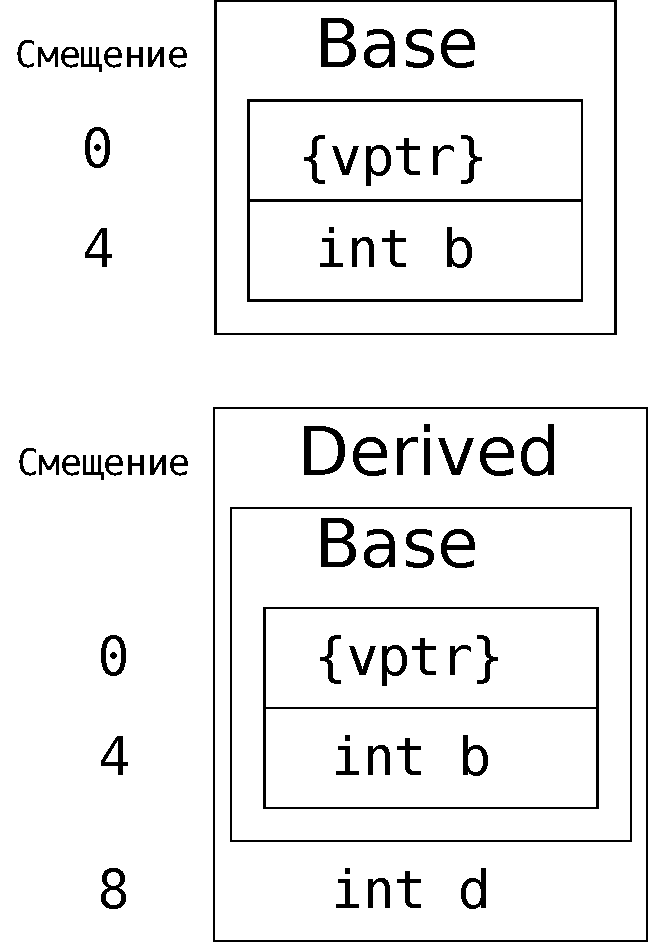
\includegraphics[width=4cm]{simple_mem_layout.pdf}
  \hfill
  \caption{Расположение классов в памяти}
  \label{memlayout_fig}
\end{figure}

\subsubsection{Расположение в памяти таблиц виртуальных функций}
Сами таблицы виртуальных функций будут иметь вид, показанный на \picref{simple_vtables_fig}
\begin{figure}
  \center
  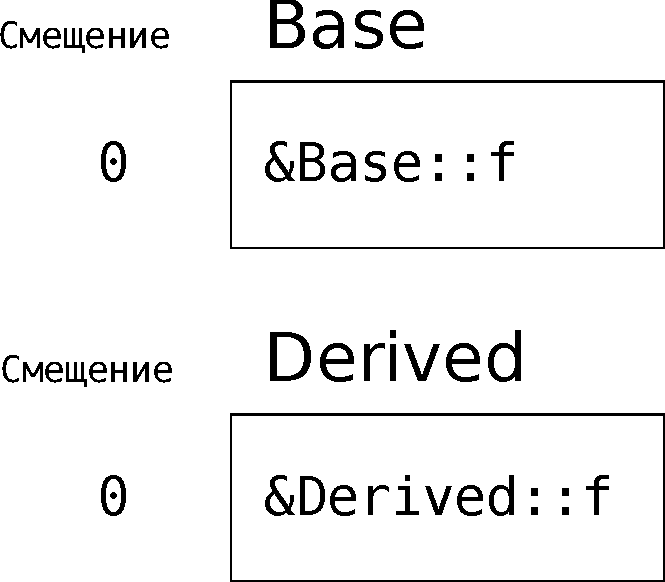
\includegraphics[width=4cm]{simple_vtables.pdf}
  \hfill
  \caption{Расположение в памяти таблиц виртуальных функций}
  \label{simple_vtables_fig}
\end{figure}

\subsubsection{Механизм виртуального вызова}
\label{virtual_call}
Вызов виртуальной функции \texttt{f} происходит следующим образом: по указателю на \texttt{base} находится указатель на таблицу виртуальных функций, из таблицы берется адрес требуемой функции, происходит вызов функции.
\begin{lstlisting}
void test(Base *base) {
  base->f();
}
\end{lstlisting}

\subsection{Метод решения задачи}
Метод решения основывается на сборе информации о имевших место вызовах виртуальных функций в программе и последующем анализе собранной информации.
Реализованный медод позволяет восстанавливать для каждого вызова виртуальной функции получать следующие значения: адрес инструкции, осуществляющей вызов, в коде программы, адрес использованной для вызова таблицы виртуальных функций и номер вызываемой виртуальной функции в таблице.
Полученная информация накапливается во время работы анализируемой программы, сам анализ проходит после её завершения.
\subsubsection{Предварительный сбор информации}
Для выявления вызовов виртуальных функций используется метод сопоставления с образцом, описанном в разделе \ref{virtual_call}.
Также должно выполняться слудующее условие: предполагаемый адрес таблицы виртуальных функций должен находиться в разделе памяти, являющимся отображением исполняемого файла и имеющего доступ только на чтение.
Для проверки этого условия множество отображений, сделанных загрузчиком программы, извлекается из виртуальной файловой системы \texttt{proc}\footnote{Информация находится в файле \texttt{/proc/\{pid\}/maps}, где \{pid\} --- идентификатор процесса.}.

Каждому адресу в коде программы, который являлся вызовом виртуальноой функции ставится в соответствие структура данных, называемая далее \emph{точкой вызова}.
В точке вызова сохраняется номер вызываемой виртуальной функции и множество таблиц виртуальных функций, использованных для вызова в этой точке.

Введем следующие обозначения.
Место вызова будем обзначать заглавной буквой, таблицу виртуальных функций маленькой.
Множество таблиц виртуальных функций, использованных в точке вызова будем обозначать $calles[A]$, номер вызываемой функции $fn[A]$.
\subsubsection{Нахождение начала таблицы виртуальных функций}
В случае, когда имеет место множественное наследование, и происходит вызов виртуальной функции одного из родительских классов, будет использоваться таблица виртуальных функций, соответствующая этому родительскому классу.
Для распознавания множественного наследования необходимо найти адрес начала таблицы виртуальных функций унаследованного класса. TODO описание метода.
\subsubsection{Построение иeрархии мест вызовов}

Алгоритм состоит из пяти фаз.
\paragraph{Продвижение множеств использованных таблиц виртуальных функций}
Пусть существуют два места вызова $A$ и $B$, при этом $callees[A] \cap callees[B] \neq \emptyset$ и $fn[A] \leq fn[B]$.
Тогда $callees[A] := callees[A] \cup callees[B]$.
\paragraph{Слияние мест вызовов}
Пусть существуют два места вызова $A$ и $B$, при этом $callees[A] \cap callees[B] \neq \emptyset$ и $fn[A] = fn[B]$.
Тогда предыдущая фаза гарантирует, что $callees[A] = callees[B]$ и два таких места вызова можно считать одинаковыми и удалить одно из них из рассмотрения
\paragraph{Сортировка мест вызовов}
Для каждого места вызова $A$ найдем множество $\mathcal{P}$, удовлетворяющее условию $\forall B \in \mathcal{P} (callees[B] \cap callees[A] \neq \emptyset) \wedge (fn[B] < fn[A])$.
Если $\mathcal{P} \neq \emptyset$, обозначим $B = arg \max\limits_{B \in \mathcal{P}}fn[B]$ (единственность $B$ гарантируется предыдущими фазами) и будем говорить, что $B$ является родителем $A$, т.е. $parent[A] := B$.

Если же $\mathcal{P} = \emptyset$, то будем говорить, что $A$ не имеет родителя.
\paragraph{Cокращение множеств использованных таблиц виртуальных функций}
Для каждого места вызова $A$ определим множество $\mathcal{P}$ как множество всех родителей $A$, т.е.\\$\{parent[A],\;parent[parent[A]],\;\dots\}$.
В частности, $\mathcal{P}$ может быть пустым.
Далее, положим $callees[A] := callees[A] \setminus \bigcup\limits_{B \in \mathcal{P}}callees[B]$.

\paragraph{Сокращение цепочек}
TODO

\subsubsection{Нахождение размера таблицы виртуальных функций}
Метод решения основывается на анализе таблиц виртуальных функций, а также динамическом анализе потока данных и потока управления.
Принадлежность класса к одной из иерархий можно установить по его указателю на таблицу виртуальных функций.
Однако, равенство указателей на таблицы виртуальных функций не будет означает однозначную принадлежность объектов к одному классу.
Возможна ситуация, когда класс-наследник не переопределяет никаких виртуальных функций.
В этом случае, таблицы виртуальных функций у классов будут одинаковыми.

Принадлежность классов к одной иерархии можно установить, анализируя виртуальные вызовы в программе.
Легко видеть, что все объекты, виртуальные методы которых вызывались одной и той же инструкцией должны принадлежать к одной иерархии классов, и этот вызов происходит через указатель на один из базовых классов. Сравнивая размеры предполагаемые размеры таблиц виртуальных функций можно установить порядок наследования классов.
Анализируя места вызова методов классов можно установить какие из них являются закрытыми (\texttt{private}), т.к. такие методы будут вызываться только из методов соответствующего класса.

%\addcontentsline{toc}{section}{Заключение}
\newpage
\section{Экспериментальные результаты}
\section{Заключение}


%% Надо вывести все рисунки до списка литературы
\clearpage

\newpage
\addcontentsline{toc}{section}{Литература}
\begin{thebibliography}{9}

    \bibitem{valgrind} Nicholas Nethercote. Julian Seward. Valgrind: A Framework for Heavyweight Dynamic Binary Instrumentation. Proceedings of ACM SIGPLAN 2007 Conference on Programming Language Design and Implementation (PLDI 2007), San Diego, California, USA, June 2007.

    \bibitem{abstracttypes} Philip J. Guo. Jeff H. Perkins. Stephen McCamant. Michael D. Ernst. Dynamic Inference of Abstract Types. Proceedings of the 2006 international symposium on Software testing and analysis.

    \bibitem{typechecking} Michael Burrows. Stephen N. Freund. Janet L. Wiener. Run-Time Type Checking for Binary Programs. International Conference on Compiler Construction, 2003.

    \bibitem{cppvg} \texttt{http://code.google.com/p/data-race-test/wiki/cpp\_vg/}
    \bibitem{strstr} Бьерн Страуструп. Язык программирования С++. М.: Бином, 2006. 1100 с.
    \bibitem{reversing_cpp}P. Sabanal, M. Yason. Reversing C++. Black Hat DC. 2007.
    \bibitem{real_decomp} M. Van Emmerik, T. Waddington. Using a decompiler for real-world source recovery. Proceedings of 11th Working Conference on Reverse Engineering, с. 27-36. 2004.
    \bibitem{boomerang} \texttt{http://boomerang.sourceforge.net/}
    \bibitem{ida_pro} \texttt{http://www.idapro.com}
\end{thebibliography}


\end{document}

%rtti
%ооп
%vtable
%this
%abi
%отношение ассоциации (uml)
%поток данных
%поток управления
%алиас
%статический анализ
%динамический анализ
